%!TEX root = main.tex

\chapter{Animations}

All animations in the project are realized in the JavaScript code and implemented as \texttt{BABYLON\\.Animation} objects, which are part of Babylon's own set of features for animation. We also use a simple wrapper library to simplify the handling of such objects.

\section{Our animation.js library}

In order to simplify the handling of the animations in our code, we wrote a small wrapper class for the Babylon Animation object. We called our new wrapper class Animation as well.

The main purpose of our wrapper is to save the length of the Babylon Animation it contains. Our module then offers a number of functions that take our wrappers as inputs and executes the contained Babylon animations by automatically setting the animation range based on the stored length. In this way we did not have to update the animation range of all function calls that execute a certain animation whenever we wanted to change the length of that animation.


\section{Character animations}

In our project we prototyped the animations in Blender. We use the keyframes values, obtained by manually manipulating the meshes using Blender tools, as reference to implement each animation in the code. After that we fine-tuned again their values to better adapt them to the scene. In order to make Blender references closest to the Babylon system, we had to set up the former to use the same order of Euler angles as Babylon, which was observed to be ZXY.

Although we always worked with Euler angles in Blender, when defining the final animations in the code we made use of both quaternions and Euler angles. The angles are used for simplicity when only a single component of the rotation vector changes, as well as a few instances where interpolating the angles worked better, while for animations that involved more than one Euler angles we decided to animate quaternions in order to get a more natural trajectory and avoid gimbal lock. We used the \texttt{BABYLON.Quaternion.FromEulerVector} function to convert between Euler and quaternions.

To animate the different meshes we use both \texttt{TransformNode} and \texttt{Bone} objects. Specifically, changes in the configuration of a node are persistent, so we used them when we wanted the final state of the object to be persistent, while the configuration of a bone is immediately reset to that of the corresponding node as soon as the animation ends for any reason. Furthermore, sometimes it happened that using the bones during the animation, the character would return to his initial position for a fraction of a second, also in this case we have worked around the problem using the nodes.
Generally, for the attacks we usually used the bones, while for animations such as Idle or Win we chose the nodes.

In order to easily access the relevant nodes and bones of the complex models, we created a JS object for each mesh to serve as a dictionary of bones for that mesh: they have the names of the relevant bones as keys and the corresponding \texttt{Bone} objects as values. Those objects can then be used to animate their rotation angles or quaternion, or retrieve the corresponding \texttt{TransformNode} object and do the same.

To finish most of the animations, we have applied some \textit{easing functions}. These allow us to define the progress rate of the animation between its beginning and its end, allowing us to speed it up or slow it down in some of its points. Most of the easing functions that we applied are quadratic or sine. Other, more peculiar easings will be pointed out explicitly below.

In the following sections we will describe the animation of each character.

\textit{\textbf{Note:} When executing a special action for the first time in each battle, the application may lag because of some initialization of the objects and particles involved, which the Babylon engine only performs at the time these elements are first used. This may prevent the animation from being shown cleanly the first time, but subsequent uses of the same special move will function normally.}



\subsection{Makoto}

\begin{wrapfigure}[14]{r}{0.5\textwidth}
    \centering
    \subfloat{
        \includegraphics[width=0.5\textwidth]{images/ch5/fireball.png}
    }
    \caption{Makoto casts Fireball}
    \label{fig:fireball}
\end{wrapfigure}

Makoto presents nine animations, four of them regards the actions that the user can takes on the battle (attack, fireball, charge, prayer), four more regard the passive movements in the battlefield (idle, flinch, death and victory) while the last one is appreciable at the end of game.



\begin{itemize}
    \item \textbf{Idle:} This animation is active when the character is not doing or undergoing any particular action and as long as this is true, the animation is repeated in loop. For Makoto, Idle consists of flexing his legs slightly, while his right leg moves forward and his left leg slightly backward.
    
    \item \textbf{Attack:} This is a simple animation, Makoto will swing his sword from the left to the right, twisting the torso in the meantime. This is a very quick animation, because it is meant to be used many times during the fight.
\end{itemize}

\begin{itemize}
    \item \textbf{Charge:} During this animation, Makoto stops moving his legs and moves its sword into a defensive position.

    \item \textbf{Fireball:}\footnote{This attack is referred to in the code with its work-in-progress codename, "Agi", which also has the benefit of being shorter and leaving the name "fireball" free for the sphere mesh to take.} This is a fairly long animation. The hero charges the magic by rotating the torso and right arm to the left, while the ambient light is lowered. When the shot is ready the character extends his arm towards the enemy and a fireball is thrown towards it (\autoref*{fig:fireball}). The fireball is a simple sphere, a Babylon primitive, with an emissive texture depicting the Sun on top. A light source moves along with in order to let the fireball light up the surrounding environment as well. When the fireball hits the enemy, it will explode. The explosion of fire is represented by the Particle System feature of Babylon, with a suitable fire-effect texture. During the animation the fireball's light will be the strongest active light source, making the animation really suggestive. At its end, the ambient light will return to normal.
    
    \item \textbf{Prayer:}\footnote{This attack is referred to in the code with its work-in-progress codename, "Dia", which also has the benefit of being shorter.} This, like Fireball, is a special animation, and to underline it also here we will see the ambient light decrease in intensity during its execution and return to normal at its end. To perform the animation Makoto will join hands, rotating his sword with the tip downwards (both for style reasons and to avoid penetration) and after that he will raise his head slightly upwards. At this point, particles will come out of the ground upwards, while healing light envelops Makoto and the ground below. Here, too, to simulate the effect of the cure, a bright green texture was applied over the particles.
    
    \item \textbf{Flinch:} This animation happens when the hero is hit by any attack and is not in a defensive position. It is quite short, both because it is designed to be reproduced often in battle, but also to simulate the quick reaction to the pain caused by the blow suffered. Makoto during Flinch will vibrate from the recoil, and will bend his torso and arms back towards his right shoulder. His head is also brought back slightly. However, the hero will quickly return to the starting position. The progression of the animation is driven by the easing function named \texttt{BackEase} with easing mode \texttt{EASEOUT}, with the result that Makoto will slightly overshoot the idle pose when returning from the flinching one, in order to show that regaining composure after being hit takes just a little more time.
    
    \item \textbf{Victory:} This animation is triggered whenever the player wins a battle. Makoto performs a final sword slash at nothing, and then puts his right hand in his pocket.
    
    \item \textbf{Death:} When Makoto loses a battle, he will first drop to his knees and then fall face down lifeless to the floor. It is a very simple animation, however, as in other animations, we refined it using the easing technique. In particular we used the \texttt{EASEIN} mode to give each part of the motion a slow, hesitant start (Makoto progressively losing his strength) and an abrupt stop (impact with the ground).
    
    \item \textbf{Ending animation:} At the end of the game, in front of his prize, we will see Makoto jump for joy on the spot. The character is translated upwards, reproducing a simple jump. The lower legs are bent back, the chin is raised slightly, the arms are raised to cheer, and to make the movement more natural, the back is bent slightly backward. All components are returned to the initial situation upon landing.

\end{itemize}



\subsection{Samurai}

This character has five animations: two attacks (normal attack, Luna special attack) and three other motions on the battlefield (idle, flinch, death).

\begin{itemize}
    \item \textbf{Idle:} A looping animation for when the Samurai is not undertaking any other action. Like Makoto, the animation consists in a little leg squatting, but to differentiate the two swordfighters, the Samurai holds his sword with two hands and in a different stance.
    
    \item \textbf{Attack:} A simple and quick animation in which the Samurai swings his katana to attack Makoto. It also twists its torso to make the hit a little more powerful.
    
    \item \textbf{Luna:} This attack has no displayed name, so it will be referred to by the name it was given in the code. The Samurai moves its sword precisely in front of it while the environmental light is dimmed to emphasize the upcoming lighting effects, and the sword and the decoration on top of the Samurai's helmet start glowing. Then the enemy raises his blade and quickly performs a downward slash, which causes an energy shockwave shaped like a crescent moon to be fired towards Makoto. When it hits, it triggers a particle effect representing the energy released by the hit and continues on its path, disappearing moments later. The projectile has an associated light source, allowing it to emit its own light and cast long shadows of the two combatants. At the end of the attack, the ambient lighting is restored.
    
    \item \textbf{Flinch:} A quick animation that triggers whenever the Samurai is hit by an attack. The enemy vibrates and recoils back, its secondary hand temporarily losing grip on the sword. Then, the warrior returns to its default position, with a little further recoil given by the \texttt{BackEase} transition function.
    
    \item \textbf{Death:} Triggers when the enemy loses all its HP. The Samurai falls to the ground in an elaborate but quick motion and dies unceremoniously.

\end{itemize}

\begin{figure}[H]
    \centering
    \subfloat{
        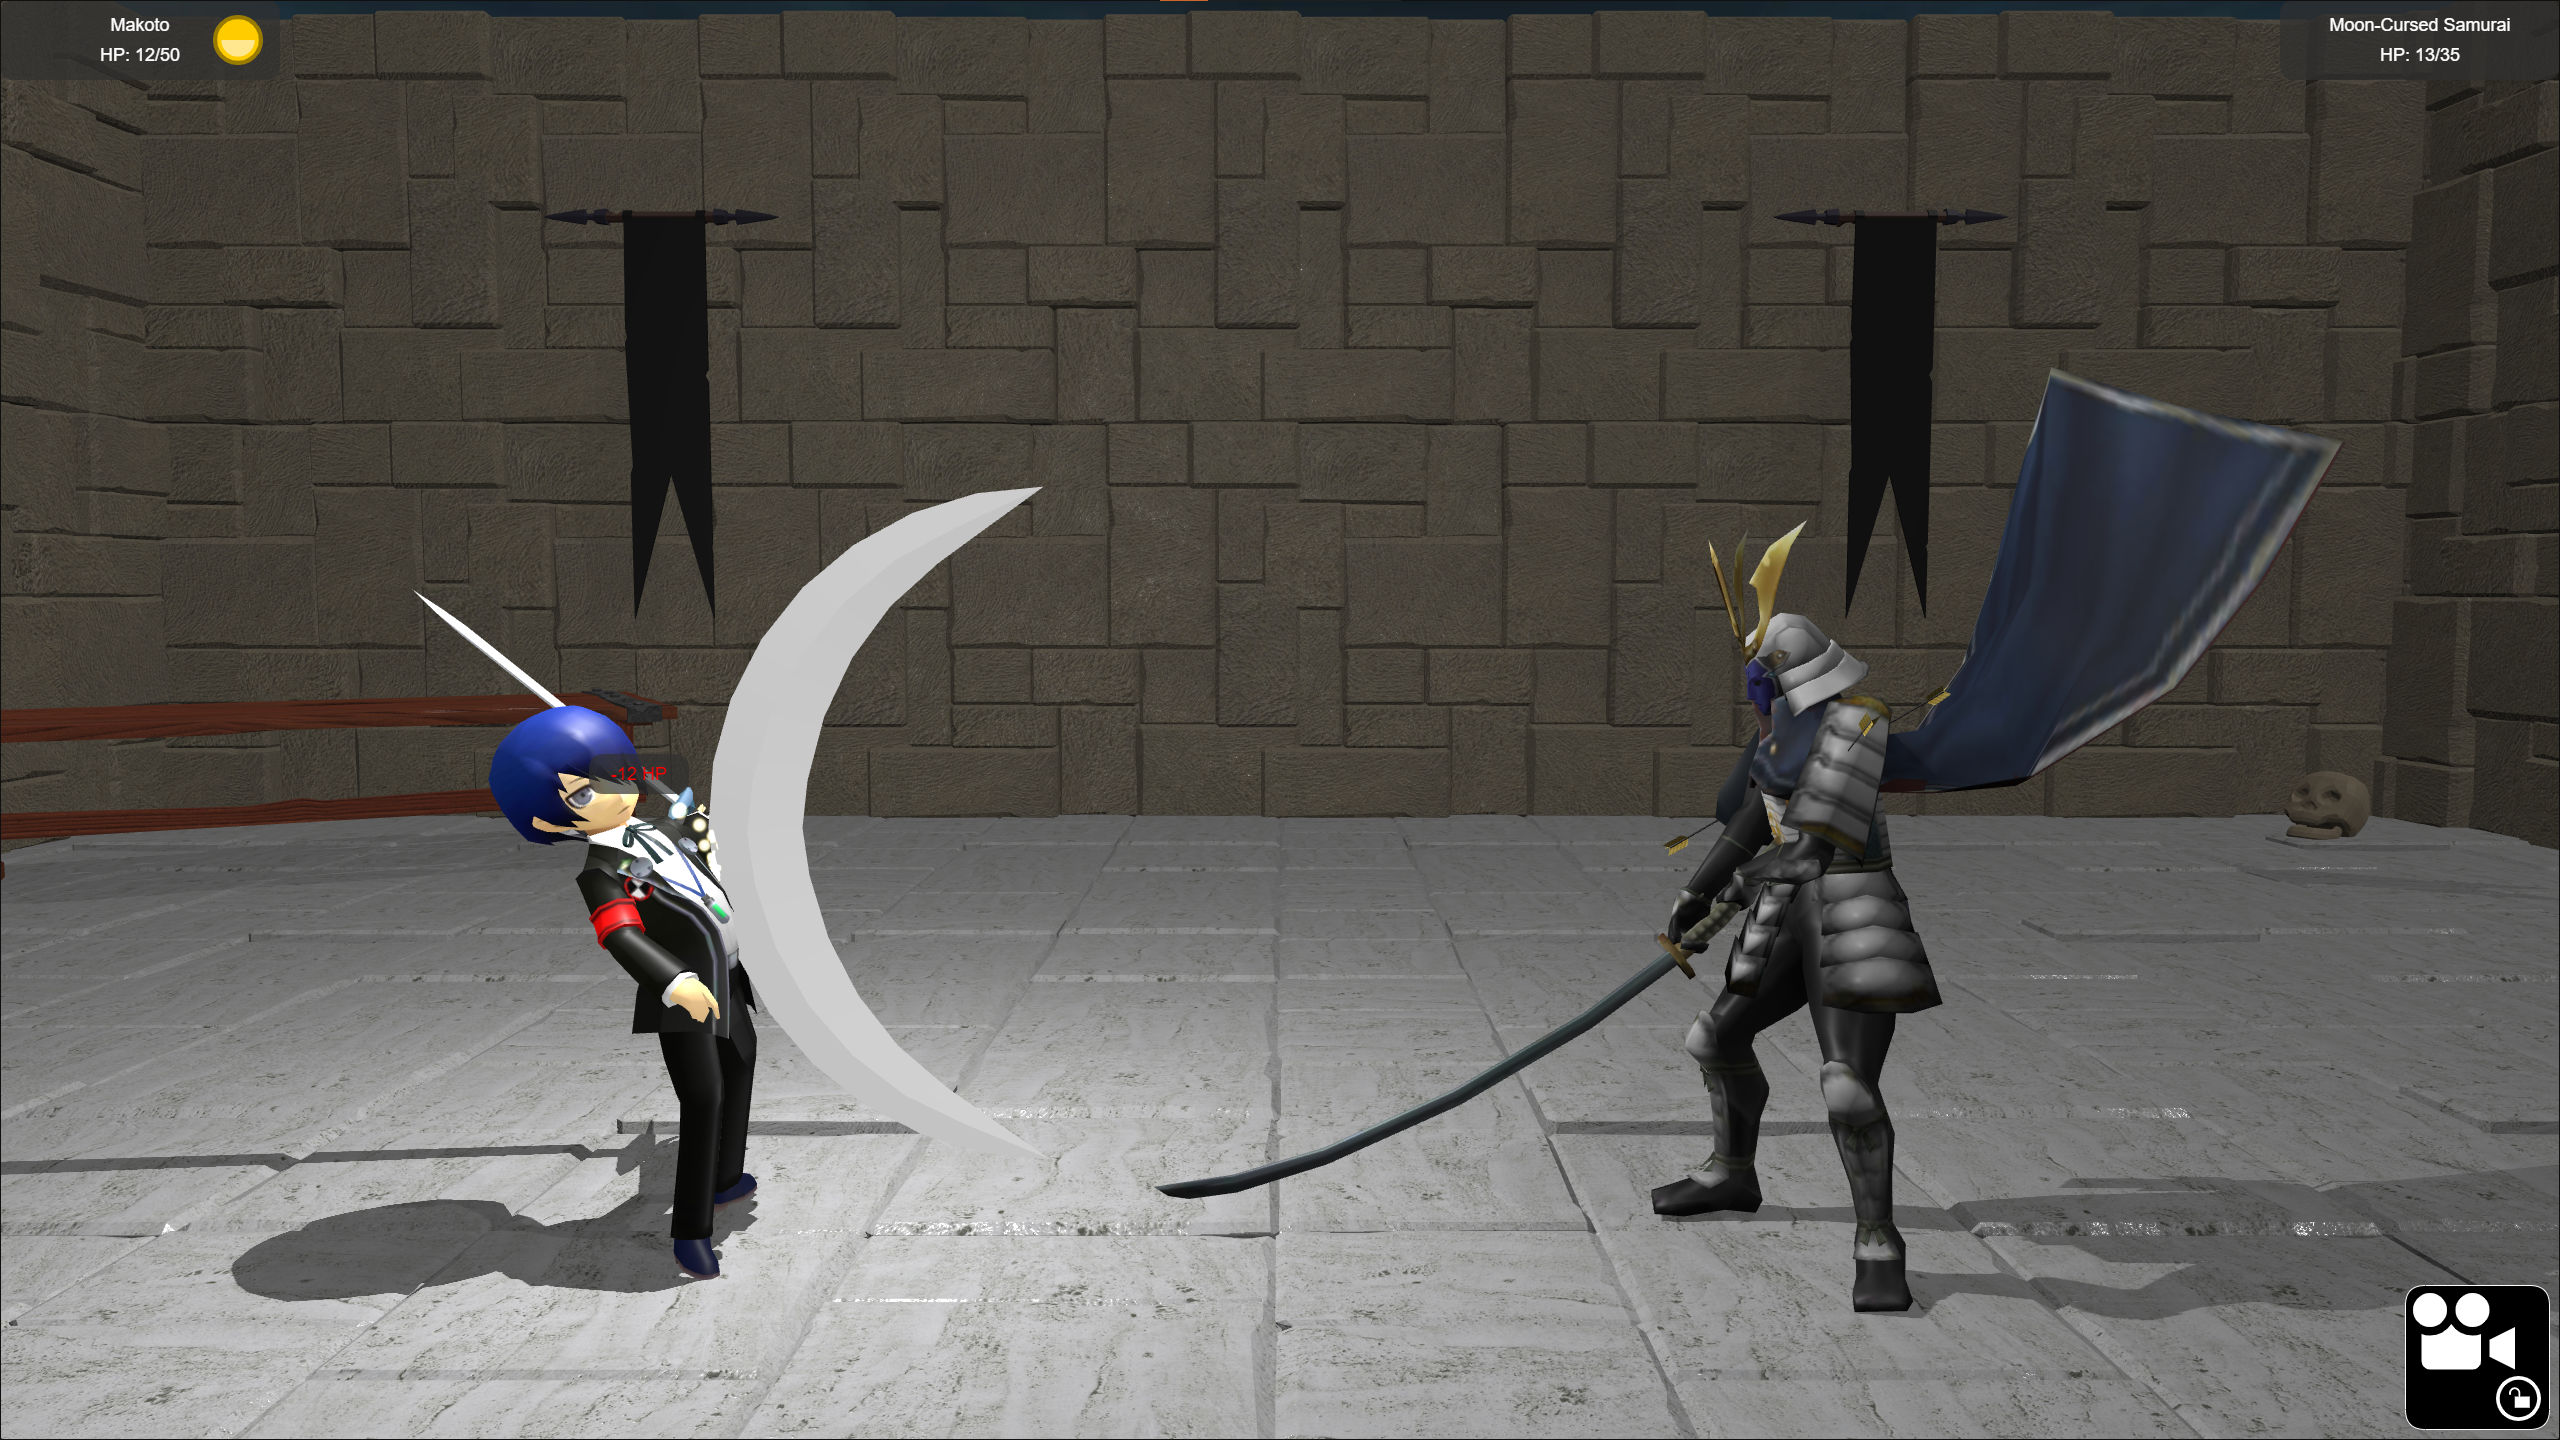
\includegraphics[width=0.7\textwidth]{images/ch5/luna.png}
    }
    \caption{Samurai attacks with Luna.}
    \label{fig:luna}
\end{figure}



\subsection{Boss}

\begin{wrapfigure}[19]{r}{0.5\textwidth}
    \centering
    \subfloat{
        \includegraphics[width=0.5\textwidth]{images/ch5/laser2.png}
    }
    \caption{The Boss attacks with its laser.}
    \label{fig:laser}
\end{wrapfigure}

This character has five animations: two attacks (normal attack, Laser special attack) and three other motions on the battlefield (idle, flinch, death).

\begin{itemize}
    \item \textbf{Idle:} A looping animation for when the Boss is not undertaking any other action. It simply consists of the monster's cape slightly expanding and shrinking in a breathing-like motion.
    
    \item \textbf{Attack:} A simple and quick animation for the normal attack. The demon raises the right side of its cape, then performs a sweeping motion with it and twists its equivalent of a spine to attack Makoto with the unnaturally sharp ends of the cape. The extremity of the cape also extends a little, in order to actually hit Makoto (rather than just performing the slashing motion and hit abstractly like the other characters do).
\end{itemize}

\begin{itemize}
    \item \textbf{Laser:} This attack has no displayed name, so it will be referred to by the name it was given in the code. After a few moments of concentration while the ambient light dims, the Boss opens its cape wide and bends forward in order to fire a laser beam from its mask. The laser pierces through Makoto, releases a particle effect, and emits light, casting the hero's shadow on the ground. At the end of the attack, the laser vanishes and the ambient lighting is restored.
    
    \item \textbf{Flinch:} The animation for when the enemy is hit by an attack. The Boss bends its equivalent of a spine backwards and sideways, while its cape opens as a result of this motion. Then the monster returns to its idle pose, with the usual recoil due to the \texttt{BackEase} effect.
    
    \item \textbf{Death:} Performed when the fiend is finally slain. An elaborate and dramatic animation: the Boss first recoils slightly in disbelief of its defeat, then it slowly starts to fall backwards as it stretches out its hand and its cape spreads wide; finally, after slowing down the motion for further dramatic effect near the end, the demon's body hits the ground, the stretched arm falls lifeless to its chest and the cape completes its fall.
\end{itemize}


\subsection{Closing note on character animations}

In order to allow each non-idle, non-flinch animation of a character to assume they will all start from the same initial pose without having the model abruptly snap to that starting pose with no transitions, those animations are only permitted to start between the end of an idle cycle and the beginning of the next one.

This means that between the moment the user clicks an action button (or the enemy starts its turn) and the moment the character performs their action there may be some waiting time depending on how close the current idle cycle is to ending, which is the cost we chose to pay in order to avoid the aforementioned rough transition. The wait can never exceed 1.6 seconds, the duration of one cycle.



\section{Other Animations}
In the \textit{dungeon} we have implemented some animations to make the game experience more dynamic and enjoyable. We have focused our attention on the principal objects present in the rooms.

\subsection{Keys and Padlock}

The animation of the keys is the first we encounter during the game. In its initial state, a key performs a simple floating animation like many other collectible objects in similar games do.

When the user interacts with the key by approaching and clicking it, the key will perform a simple transition animation to move in front of the camera and on the right side of the screen, as an object held by the player. The key remains in the same position and orientation relative to the camera as long as it is carried by the player: on the right side of the screen, very close to it to avoid penetration with the walls, and scaled down by a little to fit inside the screen.

Then, the user can use the key they are carrying on a padlock of the same color. When they do, a new animation is triggered, in which the key first flies to the lock, then turns to unlock the gate, then finally key, lock and gate bars all sink below the ground and disappear: the gate has been opened.

\begin{figure}[H]
      \centering
      \subfloat{
        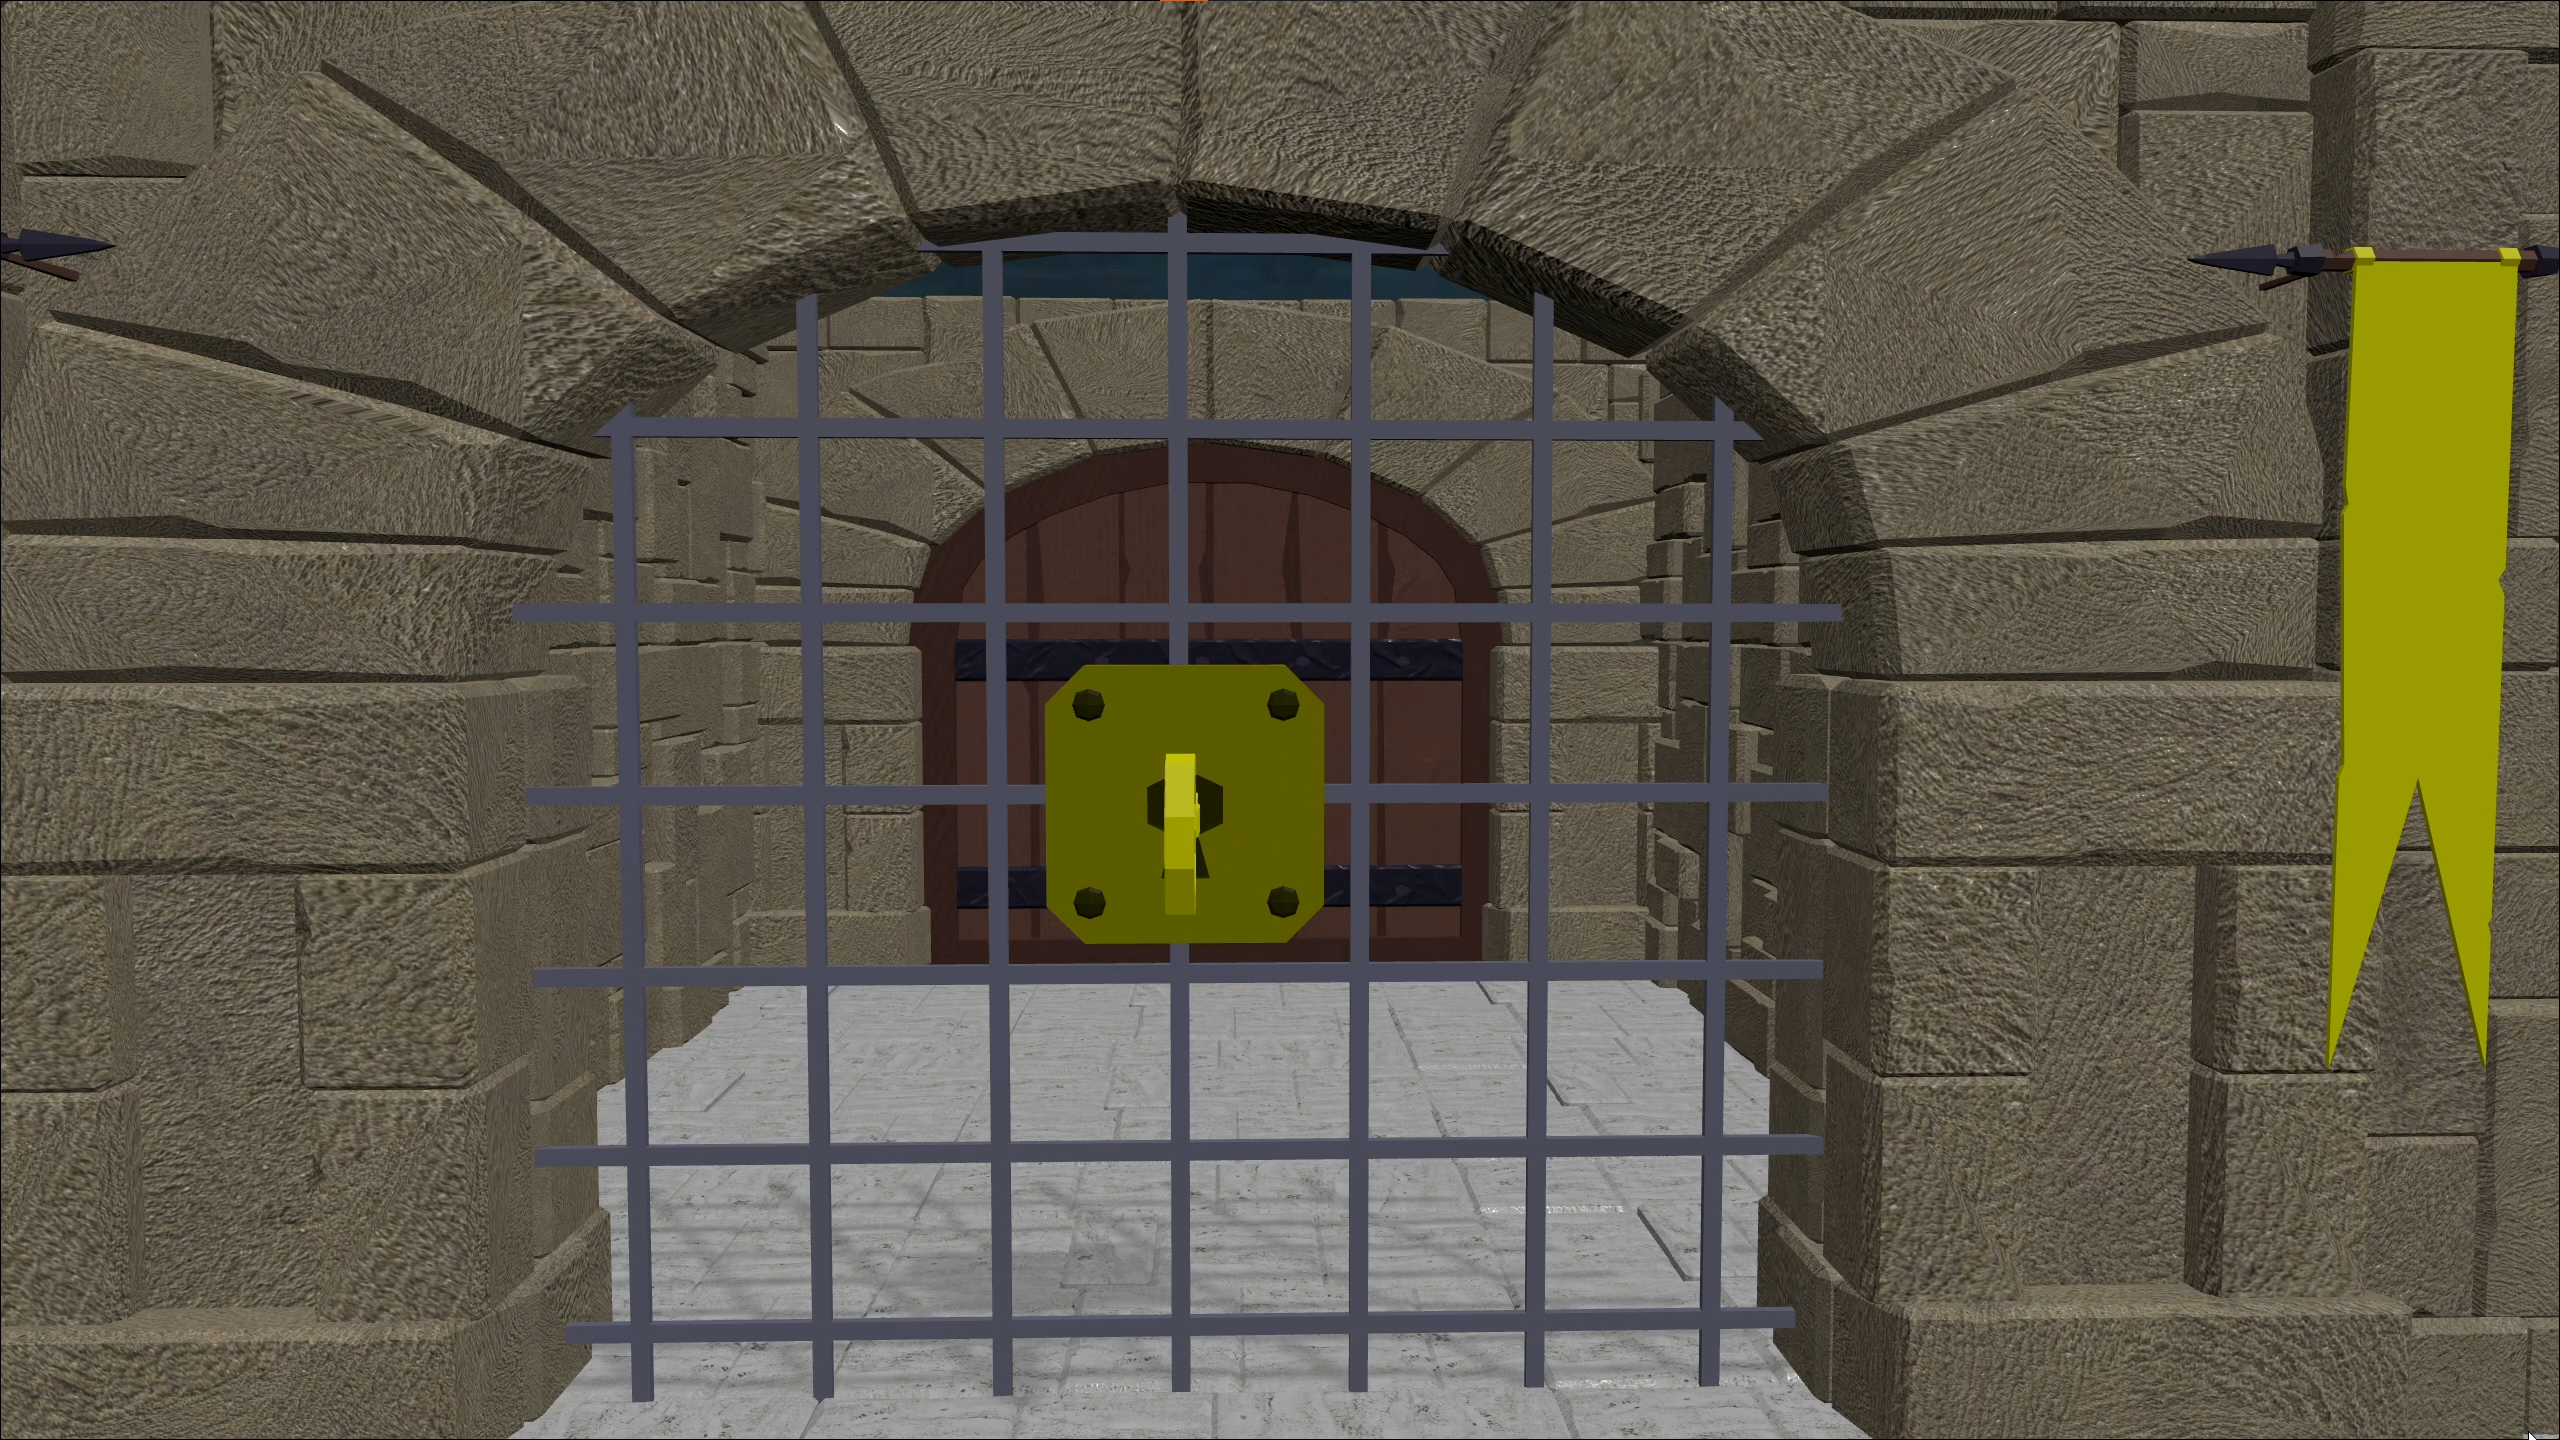
\includegraphics[width=0.4\textwidth]{images/ch5/key1.png}
    }
    \hspace{1cm}
    \subfloat{
        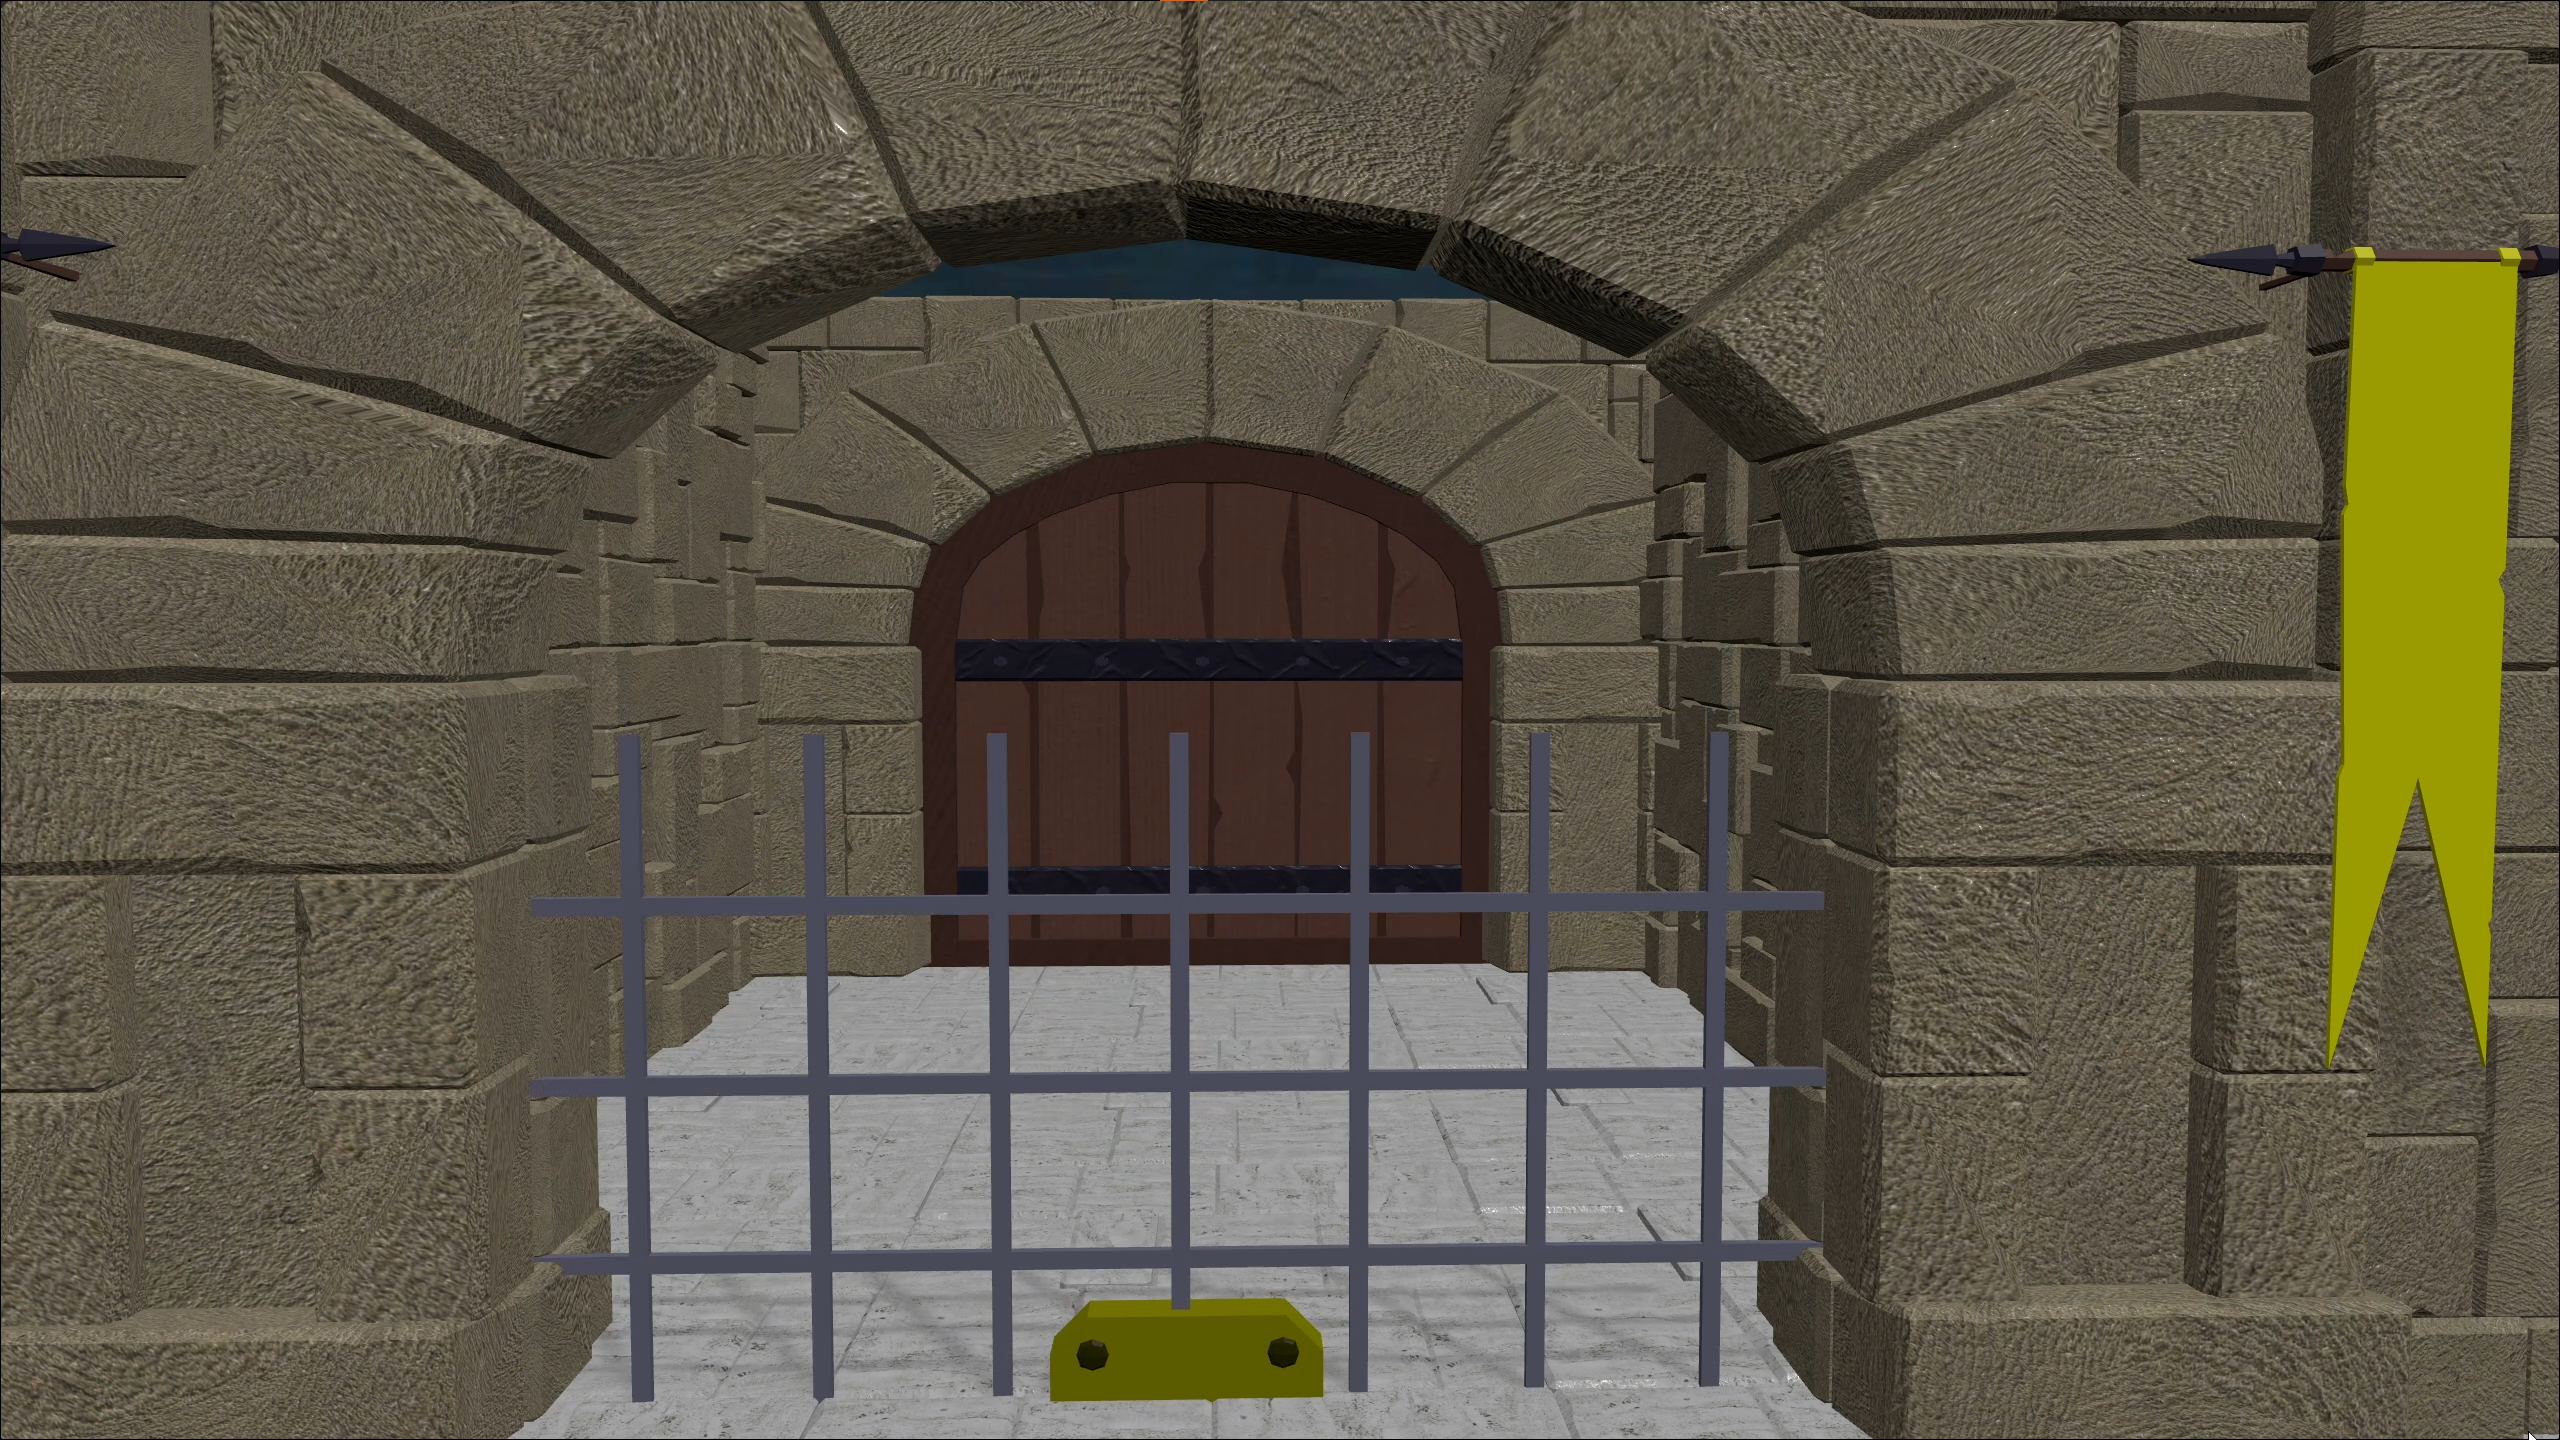
\includegraphics[width=0.4\textwidth]{images/ch5/key2.png}
    }
    \caption{Gate animation}
\end{figure}

\subsection{Door}

\begin{wrapfigure}[13]{r}{0.5\textwidth}
    \centering
    \subfloat{
        \includegraphics[width=0.5\textwidth]{images/ch5/door_open.jpg}
    }
    \caption{Door animation}
    \label{fig:door}
\end{wrapfigure}

Doors are the means by which the player moves between the different areas of the dungeon.

The animation of the door is very simple: when the user approaches and clicks it, the door swings open by rotating 90 degrees around its pivot. At the end of the animation, a scene change function is called to transport the user to the connected area.

Note, however, that in order to be able to approach certain doors the player will first have to unlock any intervening gates.


\subsection{Spike trap}


The purpose of this object is to serve as a surprise obstacle that activates when the user attempts to approach it, so that they are forced to take the detour route. It is \textit{not} intended to be a threat to the player's health. The spikes have two simple animations:

\begin{itemize}
    \item When the player comes closer than a set distance (presumably because they were trying to get to the key on the other side), the spikes will emerge from the ground in a very fast animation that uses a quintic easing function in order to be even faster.
    \item When the player takes the blue key, the trap is deactivated permanently, so the spikes sink back into the ground if they were up.
\end{itemize}

\begin{figure}[H]
    \centering
    \subfloat{
        \includegraphics[width=0.45\textwidth]{images/ch5/trap1.jpg} \hspace{5pt}
        \includegraphics[width=0.45\textwidth]{images/ch5/trap2.jpg}
    }
    \caption{spike trap before and after}
    \label{fig:trap1}
    \label{fig:trap2}
\end{figure}



